\section{Auswertung}
\label{sec:Auswertung}

\subsection{Vorbereitungsaufgabe} % (fold)
\label{sub:Vorbereitung}

In Vorbereitung auf den Versuch wird herausgesucht bei welchen Energien die Cu-$K_\alpha$- und die Cu-$K_\beta$-Linien
zu erwarten sind und bei welchen Winkeln $\theta$ sie bei Verwendung eines LiF-Kristalls ($d = \qty{201.4}{\pico\meter}$) liegen.
Die Energien liegen bei $E_{K_\alpha}= \qty{8.05}{\kilo\electronvolt}$ und $E_{K_\beta}= \qty{8.91}{\kilo\electronvolt}$\cite{X-Ray}.
Durch Umstellen von \autoref{eqn:Bragg} zu
\begin{align}
  \theta = \arcsin{\frac{h \cdot c} {E \cdot 2 d}} \label{eqn:theta}
\end{align}
wird der Glanzwinkel berechnet zu $\theta_{K_\alpha}= \qty{22.48}{\degree}$ und $\theta_{K_\beta}= \qty{20.21}{\degree}$.

Zudem wird die Ordnungszahl und Energie der K-Kante für die zu untersuchenden Materialien harausgesucht. Mithilfe von
\autoref{eqn:theta} wird der Glanzwinkel bestimmt und mithilfe von \autoref{eqn:sigmak} die Abschirmkonstante berechnet.
Die Ergebnisse sind in \autoref{tab:Vorbereitung} aufgetragen.

\begin{table}[H]
  \centering
  \caption{Literaturwerte und daraus berechnete Größen verschiedener Elemente.\cite{X-Ray}}
  \label{tab:Vorbereitung}
  \sisetup{table-format=2.2}
  \begin{tabular}{c S[table-format=2.0] S S S[table-format=1.2] }
  \toprule
  {Element} & {Z} & {$E_{K}^{lit} [\si{\kilo\electronvolt}]$}& {$\theta_{K}^{lit} [\si{\degree}]$} & {$\sigma_K$}\\
  \midrule
    Zn & 30 &  9.65 & 18.60 & 3.56 \\
    Ge & 32 & 11.11 & 16.08 & 3.66 \\
    Br & 35 & 13.48 & 13.20 & 3.84 \\
    Rb & 37 & 15.21 & 11.68 & 3.93 \\
    Sr & 38 & 16.12 & 11.01 & 3.98 \\
    Zr & 40 & 18.01 &  9.84 & 4.08 \\ 
  \bottomrule
  \end{tabular}
\end{table}
% subsection  (end)

\subsection{Überprüfung der Bragg-Bedingung} % (fold)
\label{sub:Bragg_aus}
Die Messung wird nach \autoref{sub:Bragg_durch} durchgeführt.
Aus den gemessenen Daten wird das Maximum der Kurve bestimmt und mit dem Sollwinkel verglichen.
\begin{figure}[H]
  \centering
  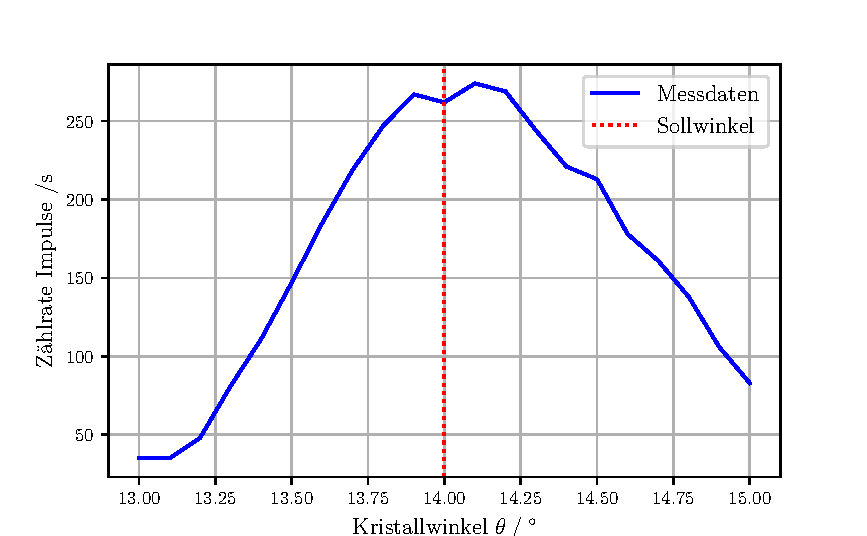
\includegraphics[width=\textwidth]{build/plot1.pdf}
  \caption{Emissionsspektrum bei festem Kristallwinkel von $\theta = \qty{14}{\degree}$.}
  \label{fig:plot1}
\end{figure}

Das Maximum der Kurve in \autoref{fig:plot1} liegt bei $2*\theta=\qty{28.2}{\degree}$, bzw. bei $\theta=\qty{14.1}{\degree}$.

% subsection Überprüfung der Bragg-Bedingung (end)

\subsection{Analyse des Emissionsspektrums einer Cu-Röntgenröhre} % (fold)
\label{sub:Emission_aus}

\begin{figure}[H]
  \centering
  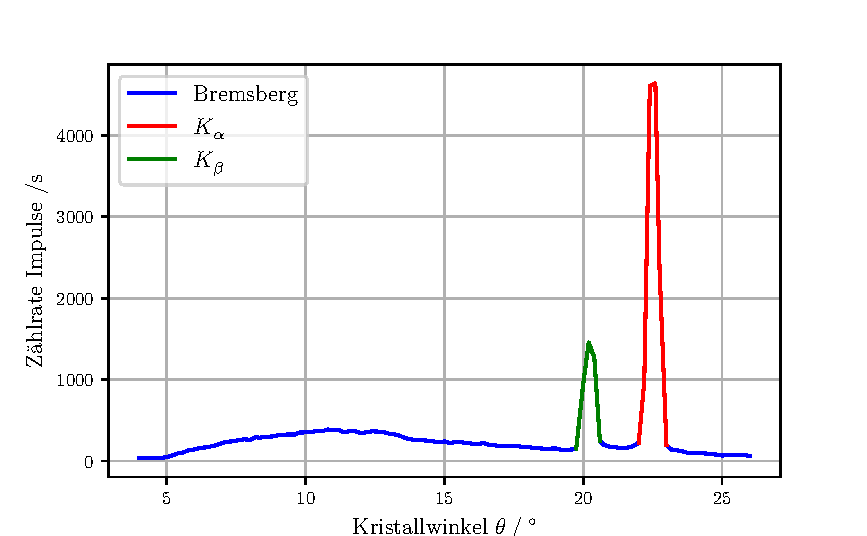
\includegraphics[width=\textwidth]{build/plot2.pdf}
  \caption{Emissionsspektrum der Cu-Röntegnröhre.}
  \label{fig:plot2}
\end{figure}

Die Maxima der Kurve und somit die Winkel für die Energien liegen für die 
$K_\alpha$ -Energie  bei $\theta_\alpha=\qty{20.2}{\degree}$ und für die $K_\beta$ - Energie
bei $\theta_\beta=\qty{22.6}{\degree}$.



% subsection Das Emissionsspektrum einer Cu-Röntgenröhre (end)

\subsection{Analyse der Absorptionsspektren} % (fold)
\label{sub:Absorption_aus}

Zink Maximum bei 18.9 Minimum 18.2
Strontium Maximum 11.3 Minimum 10.5
Zirkonium Maximum 
% subsection Das Absorptionsspektrum (end)